\documentclass[sigconf,anonymous=false]{acmart}

%\fancyhf{} % Remove fancy page headers 
%\fancyhead[C]{Anonymous submission \#9999 to ACM CCS 2019} % TODO: replace 9999 with your paper number
%\fancyfoot[C]{\thepage}

%\setcopyright{none} % No copyright notice required for submissions
%\acmConference[Anonymous Submission to ACM CCS 2019]{ACM Conference on Computer and Communications Security}{Due 15 May 2019}{London, TBD}
%\acmYear{2019}

\settopmatter{printacmref=false, printccs=false, printfolios=false} % We want page numbers on submissions
\definecolor{Orange}{rgb}{1,0.5,0}
\usepackage{xcolor}
\newcommand{\todo}[1]{\textsf{\textbf{\textcolor{Orange}{[[#1]]}}}}
\usepackage{graphicx} %Loading the package
\graphicspath{{../measurement/results/}}
\usepackage{booktabs}

\begin{document}
\title{Measuring How Much IoT Devices Upload via Traffic Analysis} % TODO: replace with your title
\author{Enze Liu, TJ Smith, Zesen Zhang}
%\orcid{0000-0000-0000}
\affiliation{%
  \institution{University of California, San Diego}
}
\email{{e7liu, tjs003, zez003}@eng.ucsd.edu}

\begin{abstract}
Smart speakers, such as Amazon Echo, have gained popularity in recent years. These smart speakers normally have always-on microphones that are used to detect voice commands. While being useful, this behaviour of constantly listening has raised a wide range of privacy concerns. These include, but are not limited to, what is being recorded, how the collected data is used and stored, and whether it is being protected well. In this work, we quantitatively answered two frequently asked privacy-related questions about Amazon Echo. First, does it stream any conversation before it is activated? Second, is any audio being sent after Echo detects the end of a command? We designed and performed measurements that allowed us to answer these two questions. We first confirm that usually Echo is not transmitting any audio that happens before it is activated. We further verify that in the case of correctly detecting the end of a command, Echo will not stream any conversation that occurs after the command. Additionally, we are able to quantify that a 0.7 second gap is needed for Echo to correctly detect the end of a command. While there is a rich literature on analyzing Echo's network traffic, ours is the first to use its network traffic to answer the two questions aforementioned in a quantitative manner.
%To achieve this, we prerecorded a piece of audio that contained an Echo command ("Alexa, where is New York City?") as well as irrelevant conversations prefixing and suffixing the Echo command. Different segments of this audio were played over and over again in a controlled environment, and all packets transmitted by Echo were recorded. After data cleaning and carefully analyzing the traffic data, we are able to reveal \todo{X} key findings. First, we confirmed that normally Echo would not stream any conversation that happened before the wake word. That said, we did observe that, sporadically, Echo would transmit a non-trivial amount of data during an ongoing conversation that did not contain the wake word. \todo{What else did we find}. 
\end{abstract}

\ccsdesc{Security and privacy~Use https://dl.acm.org/ccs.cfm to generate actual concepts section for your paper}
% -- end of section to replace with generated code

%\keywords{template; formatting; pickling} % TODO: replace with your keywords

\maketitle

\section{Introduction}
Physical devices connected to the internet, also known as Internet-of-things (IoT), have gained its popularity in recent years. Among numerous types of IoT devices, smart speakers with voice assistants, such as Amazon Echo and Google Home, are widely seen in users' home. These devices would detect and respond to voice commands. They normally have always-on microphones, which theoretically would start recording after hearing a wake word and then send the voice data to a server via internet for further processing \cite{AmazonEc68:online}.

This behavior has sparked many privacy concerns, including but not limited to what is being recorded, how the collected data is used and stored, and whether it is being protected well \cite{lau2018alexa, fowler_2019, apthorpe2017smart, apthorpe2019keeping, apthorpe2017spying}. Much of previous work has been centered around protecting sensitive information from being leaked to adversaries \cite{apthorpe2017smart, apthorpe2019keeping, apthorpe2017spying}. As for what data is being collected, Amazon has made it possible for users to view, play and delete their voice data stored on its server \cite{ford2019alexa}. However, our intuition is that Amazon would reveal to users only part of the voice data being collected by its smart speakers. Up until now, little has been done to verify whether Amazon is being honest with us or not -- is Amazon making public exactly the audio data it collects?

Researchers from Princeton have successfully inferred user activity using network traffic measurement \cite{apthorpe2017spying}, building on top of which others have been able to establish network signatures for Amazon Echo's network traffic. We plan to use the same technique for our work, and it is turns out to be working, we will be able to answer a whole set of questions.
%Our expectation of Amazon Echo is that if it is given the same audio input, it should stop recording at the same place every time. Our preliminary experiments with Amazon Echo have found that the recorded voice of the same command is not consistent across different trials, suggesting something different. This stimulates us to question and examine the behavior of Amazon Echo and dig into what is exactly being collected by it. We are hoping to get some insights into this question using network traffic measurement, as previous researchers \cite{apthorpe2017spying} have successfully inferred users' activities leveraging the same technique.
\section{Background}
Amazon Echo is a smart speaker developed by Amazon that is connected to the internet~\cite{wikipedia_2019}. It has an always-on microphone that starts recording automatically after hearing certain wake word (Alexa, Echo, etc.). Voice commands following the wake word are streamed to Amazon's cloud-based intelligent command handling program, known as Alexa, for further processing. Alexa will then try to respond to users' commands. Amazon also keeps copies of the voice commands and responses, together known as response cards~\cite{ford2019alexa}. These response cards have been made available to users by Amazon so that they can be viewed, played, and deleted~\cite{amazon_2010}.
%\section{Experiment Setup}

%We will begin by measuring the baseline traffic from the smart speaker in a silent environment. This should allow us to identify the regular traffic patterns of the smart speaker when it is not transmitting voice data. %We will then test several basic pre-recorded commands with the smart speaker to identify the basic traffic signature of the speaker when it is transmitting voice data.
%
%Once we have baseline traffic patterns we will begin more detailed measurements. We will test pre-recorded commands of varying lengths many times, to establish correlations between recording length and traffic speed and/or duration. We will then repeat these tests in the presence of several different forms of background noise, including at least podcasts, music, and discussion among ourselves. %We will not perform any tests in public environments to avoid any possible ethical considerations.
%
%To determine how the speaker decides to terminate its recording, we will use several different pathological commands. We will use incomplete commands, very long commands, and commands spoken very unclearly. By correlating the traffic patterns of these commands to the more normal commands previously measured, we hope to calculate the rough length of time the recording lasts.
%
%We will obtain whatever information we can from the cloud (e.g. through an app or API) to compare such information to our traffic pattern analysis and determine whether they match within whatever margin of error we can achieve. We will also test the behavior of the speaker in noisy environments without any commands being given to determine the rate of false recordings.
%
%\subsection{Devices}
%Our main device for testing will be the Amazon Echo, as it is the most popular smart speaker.
%
%If available, we would also like to test the Apple HomePod, as Apple places a much greater emphasis on security and privacy than its competitors.

\section{Experiment}

We ran some experiments on Alexa and use Wireshark to see if Alexa recorded consumer's voice more than we suppose it does.

\subsection{Monitoring Set Up}
\label{sec:expr:set-up}

In order to catch the packets that were sent out by Alexa to the Amazon cloud server, we set up a WiFi router on a desktop server and connected the Echo to it. We run Wireshark~\cite{wireshark} on the desktop server to capture all the packets to and from the Echo speaker.

Since we cannot directly examine the contents of the packets sent to and from the Echo, as they are all encrypted by TLS, we instead must examine coarser-grained information, like packet count, packet sizes, server ip addresses, and packet timing information. Since most of this kind of coarser-grained information is subject to variation based on network conditions, and the voice data itself is subject to variation based on environmental noise, we opt to repeat all of our experiments many times (10s to 100s) to draw statistical conclusions. 

To ensure the repeatability of such experiments, we synthesize all our voice commands and play them to the Echo using the desktop server. We also use it record any response that the Echo may give, which allows us to gather all relevant data for our experiments on a single, centralized platform. Each experiment consists of some number of different voice commands that we iterate through throughout the experiment. We leave 30~s to a minute between each command to allow the Echo to reset, and after reaching the end of our set of commands, we loop back to the beginning. We perform each experiment overnight in the office, to remove any extra human noise and ensure that the Echo only responds to the commands we provide it. We interleave the commands that we are testing to make sure that any variation throughout the night due to conditions we cannot account for affect each of the commands equally.

To make analysis easier, we use the desktop server to inject markers into the Wireshark packet capture at critical moments. This allows the analysis code to read only the single Wireshark capture and still obtain all necessary information. In particular, the desktop server pings four different predefined locations (\textit{e.g.}, 8.8.8.8) at four specific times: when the command starts playing, when the command stops playing, when Alexa's response begins, and when Alexa's response ends.

\subsection{Analysis Techniques}


After an overnight run of an experiment, we programmatically divide the Wireshark capture into experiment frames (individual command trials). We define these frames using the ping packets generated by the desktop server; the extent of each frame spans from the start of the voice command to the start of Alexa's response. This captures all the data sent by the Echo to the Amazon servers and the response from the Amazon servers back to the Echo, since we know that such a response must be complete by the time the Echo speaks that response.

\begin{figure}[!t]
    \centering
    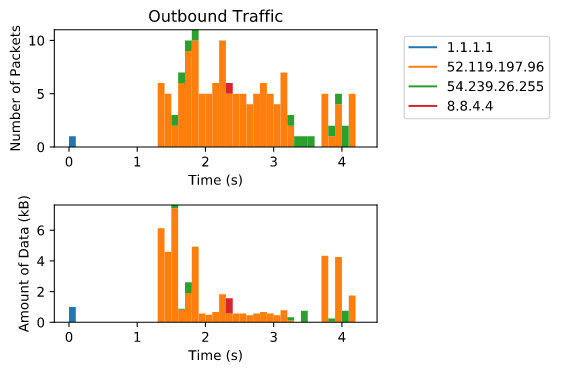
\includegraphics[width=\linewidth]{sample_hist_out.png}
    \caption{On top, time histogram of the number of packets sent from the Echo, sorted by destination IP address. On bottom, time histogram of total data sent from the Echo, sorted in the same way. The blue and red bars do not indicate real traffic, but rather mark the start and end of the command given to the Echo, as discussed in Section~\ref{sec:expr:set-up}. The time histogram ends at the moment the Echo begins its reply. The orange bars are those of the Alexa server, in this case, as they constitute by far the most data.}
    \label{fig:example_frame}
\end{figure}

The Echo communicates with many different servers for background tasks, and even a couple different servers as part of processing a command. As shown in Fig.~\ref{fig:example_frame}, though, the Echo sends the majority of its data to a single IP address, namely the Amazon server handling the Alexa request. For each frame, we choose to only count the data going to this server, as it provides the most consistent metric to compare across. The precise identity of the Alexa server changes fairly frequently, so in the course of our analyses we used two different methods to identify the server in each frame: (1) we manually inspected many packet data time histograms (as in Fig.~\ref{fig:example_frame}) to create a whitelist of Alexa serves, and (2) we simply chose the IP address in each frame that had the most data sent to it. Both methods gave very similar results, so we used the latter for most analyses, as it was more automated.

Some of the frames had much more data sent in them than others did, and inspection of their time histograms generally revealed that this was due to unusual traffic patters clearly not related to our commands (perhaps background updates or other such maintenance). These outliers needed to be filtered, as in some cases they were so high as to completely change the mean and standard variation of the entire data set. To filter such outliers, we decided to use the IQR (inter-quartile range) method to remove them. The IQR is defined as the difference of the 3rd quartile value and the 1st quartile value, and we filter any value that is more than 1.5*IQR higher than the 3rd quartile value or lower than the 1st quartile value. In other words, we keep a value $x$ only if $Q1 - 1.5*IQR < x < Q3 + 1.5*IQR$. We chose this method because of its high robustness to large outliers.

We choose to only count the data sent in TLS packets, as the Echo encrypts all of its traffic, and so any other packets are only handshakes, DNS requests, or other such administrative packets. We are careful to only count the size of the actual TLS payload, and not any of the header bytes, so as to ensure the most accurate accounting possible.




\section{Measuring traffic streamed to server}
This measures the traffic streamed to server.
\section{Conclusion And Future Work}
We have presented some of the first measurements that seek to understand the behavior of the Echo in terms of what is being transmitted by the Echo. More specifically, we found that: 1) The Echo is not usually transmitting any audio that happens before it is activated; 2) In the case of correctly detecting the end of a command, Echo will not stream any conversation that occurs after the command; 3) A 0.7~s gap is needed for the Echo to correctly detect the end of a command. While there is a large amount of research on analyzing the Echo’s network traffic, ours is the first to use its network traffic to characterize its behavior quantitatively.

Despite having some inspiring results, we did notice some apparent limitations in this work and would leave them for future work. First, we only performed the experiment with one particular command. Thus, our findings do not necessarily generalize to scenarios where other Echo commands are used. Second, we observed a few cases in all of the experiments where the amount of data transmitted was unexpected. We were unable to analyze and explain what happened as we could not decrypt the data. Finally, there is the inherent weakness of our approach---inferring the Echo's behavior by measuring its traffic. Noise and other disturbances made it harder for us to draw any conclusion statistically.
% \section{Background}
Amazon Echo is a smart speaker developed by Amazon that is connected to the internet~\cite{wikipedia_2019}. It has an always-on microphone that starts recording automatically after hearing certain wake word (Alexa, Echo, etc.). Voice commands following the wake word are streamed to Amazon's cloud-based intelligent command handling program, known as Alexa, for further processing. Alexa will then try to respond to users' commands. Amazon also keeps copies of the voice commands and responses, together known as response cards~\cite{ford2019alexa}. These response cards have been made available to users by Amazon so that they can be viewed, played, and deleted~\cite{amazon_2010}. 

\appendix

%\section{Location}

%Note that in the new ACM style, the Appendices come before the References.

%\section{Call for Papers}

The conference seeks submissions presenting novel research results in
all aspects of computer and communications security and privacy,
including both practical and theoretical contributions.

\subsection{Paper Submission Information}

Submissions must be received at \url{https://ccs17.hotcrp.com/} by the
strict deadline of {\bf 19 May 2017 at 8:59 PM PDT (UTC-7)}.
Submitted papers must not substantially overlap with papers that have
been published or that are simultaneously submitted to a journal,
conference, or workshop. Submissions must be anonymized and avoid
obvious self-references.

CCS has traditionally required that authors submitting papers
guarantee that an author will be able to present their paper at the
conference. We recognize, however, that the current travel
restrictions and screening processes may make it impossible or
uncomfortable for some authors to travel to the conference. The venue
for CCS 2017 was selected several years ago, and we do not wish to
exclude any potential authors who may have difficulty traveling due to
recent changes in US immigration practices.  CCS welcomes submissions
by authors of all nationalities, and will make allowances for
presenting papers electronically or with non-author presenters in
cases where paper authors are unable to travel to the United States.

Submissions will be evaluated based on their scientific merit,
novelty, importance, presentation quality, and relevance to computer
and communications security and privacy.  If a paper includes work
that raises ethical concerns it is up to the authors to convince the
reviewers that appropriate practices were followed to minimize
possible harm and that any harm caused by the work is greatly
outweighed by its benefits. The review process will be carried out in
two phases and authors will have an opportunity to provide a
length-limited response to the first-phase reviews.

\subsection{Paper Format}

Submissions must be single PDF files containing at most 12 pages in
the required new ACM format (see
\url{https://www.sigsac.org/ccs2017/format} for details and templates,
which you have presumably found if you are reading this!) of body
content, with any number of additional pages for the bibliography,
well-marked appendices, and any desired supplementary material.  When
relevant, submitters may include reviews from past submissions and
responses to them in the supplementary material.

Reviewers are not required to consider the appendices or supplementary
material, however, so submissions need to be intelligible and
convincing without them.  Submissions not meeting these guidelines, or
playing games to work around page limits, will be rejected by the PC
chairs without review.  In particular, papers should not use squeezing
tricks to adjust the (already very dense) ACM paper format, and moving
discussion of key related work or important definitions to appendices
may be grounds for rejection.

\subsection{Practice Talks}

Following the lead of USENIX Enigma, we want to improve the quality of
the conference and provide a better experience for both presenters and
attendees by holding practice sessions before the conference (see
\url{https://www.sigsac.org/ccs2017/practicefaq}). Presenting authors
of accepted papers are expected to participate in an on-line practice
session approximately three weeks before the conference.

\subsection{Conflicts of Interest}

The conference requires cooperation from both authors and program
committee members to ensure a process that is both fair in practice
and perceived to be fair by everyone. When submitting a paper, authors
are required to identify members of the program committee who may not
be able to provide an unbiased review.  This includes people with
strong personal or professional relationships such as advisor/advisee,
members of the same organization, and close collaborators (for
example, recent or repeated co-authors). In general, this means anyone
who a reasonable person with all the relevant information would
question as an impartial reviewer. The program co-chairs reserve the
right to request a more specific description of a conflict-of-interest
declaration from authors.

Program committee members who have a conflict of interest with a
paper, including program co-chairs, will be excluded from evaluation
and discussion of the paper, but because submissions are anonymous to
reviewers it is important for submitting authors to identify these
conflicts. In the case of a program co-chair, the other co-chairs who
do not have conflicts will be responsible for managing that paper.
Program co-chairs are not permitted to be involved as co-authors in
any submissions.




%\begin{acks}
% TODO: For the submission, don't include acknowledgments since they would most likely deanonymize you.
%\end{acks}
 % TODO: replace with your brilliant paper!

\bibliographystyle{ACM-Reference-Format}
\bibliography{iotrecording}

\end{document}
